\section{赤道波动的模态分析}
\label{sec:waves}

在第 \ref{sec:framework} 节中，我们建立了描述赤道波动的数学框架，并指出其解空间可由三个量子数 $(\vertmode, \modenum, \wavenum)$ 完全刻画。
本节将在该框架下系统地求解各类本征模态，首先在干大气情形（$\nonadheat = 0$）下显式推导垂直结构与水平色散关系，随后讨论引入非绝热加热后波动性质的修正。
前者对应于 \citep{matsunoQuasiGeostrophicMotionsEquatorial1966} 的经典理论，后者则涉及对流与动力学过程的耦合机制，是解释观测中对流耦合赤道波（CCEWs）传播特性的关键步骤。

\subsection{干大气垂直结构的显式求解}
\label{subsec:vertical_structure}

在干大气情形下，大气动力学退化为由旋转、分层和几何约束共同控制的线性系统。
对该此情况的研究不仅能够给出赤道波动的基本模态结构，而且为理解更复杂情形（如对流耦合赤道波和湿过程调制）提供了清晰的参照基准。
许多平流层和中高层对流层观测到的赤道 Kelvin 波、Rossby 波及惯性重力波，均可在这一极限下得到定量解释，因此干大气理论构成赤道波动力学的出发点。

垂直本征方程 \eqref{eq:vertical_eigen} 的显式解依赖于 Brunt-Vaisala 频率 $\bvfreq(z)$ 的具体分布形式。
为获得解析结果，这里假设 $\bvfreq = \const$，并采用背景密度随高度指数衰减的分布 \eqref{eq:background_density}。
在此假设下，本征方程可写为：
\begin{equation}
    \ode[2]{\vertfunc}{z} - \frac{1}{\scaleheight} \ode{\vertfunc}{z} + \frac{\bvfreq^2}{\gravityconst \eqdepth} \vertfunc = 0
    \label{eq:vertical_ode}
\end{equation}

引入变换 $\vertfunc(z) = \ee^{z/(2\scaleheight)} \chi(z)$ 以消去一阶导数项，代入后 $\chi(z)$ 满足标准的简谐振子方程：
\begin{equation}
    \ode[2]{\chi}{z} + \vertmode^2 \chi = 0
    \label{eq:chi_equation}
\end{equation}

其中垂直波数 $\vertmode$ 由下式定义：
\begin{equation}
    \vertmode^2 \equiv \frac{\bvfreq^2}{\gravityconst \eqdepth} - \frac{1}{4\scaleheight^2}
    \label{eq:vertical_wavenumber}
\end{equation}

式 \eqref{eq:vertical_wavenumber} 建立了等效深度 $\eqdepth$ 与垂直波数 $\vertmode$ 之间的定量联系。
垂直波数的倒数对应垂直波长 $L_z \sim 2\pi/\vertmode$，该量表征扰动在垂直方向上的特征尺度。
与均匀介质中的波数不同，此处的 $\vertmode$ 同时受稳定度 $\bvfreq$、重力加速度 $\gravityconst$ 以及等效深度 $\eqdepth$ 的共同控制。
等效深度作为连接三维垂直结构与等效浅水系统的关键参数，通过式 \eqref{eq:vertical_wavenumber} 直接决定了给定水平模态在垂直方向上的传播性质 \citep{hayashiTheoryLargeScaleEquatorial1970}。

当 $\vertmode^2 > 0$（即 $\eqdepth < \eqdepth_c \equiv 4\bvfreq^2\scaleheight^2/\gravityconst$）时，垂直波数为实数，方程 \eqref{eq:chi_equation} 具有振荡解 $\chi(z) = A\cos(\vertmode z + \varphi)$，对应于可在垂直方向上传播的内部重力波模态。
此时垂直结构函数为：
\begin{equation}
    \vertfunc(z) = A \ee^{z/(2\scaleheight)} \cos(\vertmode z + \varphi)
    \label{eq:Z_oscillatory}
\end{equation}

该解描述了一种随高度振荡、振幅指数增长的结构。
振幅的增长并不意味着能量发散，其物理原因在于背景密度随高度呈指数衰减。
能量密度 $\density_0 \abs{\vertfunc}^2 \propto \ee^{-z/\scaleheight} \cdot \ee^{z/\scaleheight} = \const$ 保持常数，从而保证了垂直传播内波的能量守恒。

相反，当 $\vertmode^2 < 0$（即 $\eqdepth > \eqdepth_c$）时，垂直波数变为纯虚数。
令 $\vertmode = \ii\mu$（$\mu > 0$），则垂直结构函数写为：
\begin{equation}
    \vertfunc(z) = \ee^{z/(2\scaleheight)} \left( B_1 \ee^{\mu z} + B_2 \ee^{-\mu z} \right)
    \label{eq:Z_evanescent}
\end{equation}

为保证解在 $z \to \infty$ 时有界，必须取 $B_1 = 0$，从而扰动随高度迅速衰减。
该类解对应于外波或俘获模态，其能量被限制在低层大气中而无法向上传播。
这种由振荡型解向指数衰减型解的转变，反映了当等效深度过大时，大气分层不足以支持波动在垂直方向上的自由传播。

\subsection{边界条件与等效深度的量子化}
\label{subsec:boundary_conditions}

垂直本征问题的谱结构不仅由大气分层性质决定，还关键性地依赖于所施加的边界条件。
不同的垂直边界假设对应着不同的物理情景：刚性边界描述了垂直运动受限的大气柱，而辐射边界则允许波动能量向高空泄露。
边界条件直接决定了等效深度是否形成离散模态谱，进而影响赤道波动在垂直方向上的尺度选择及其水平传播特性。

在地表 $z=0$ 处，不可穿透条件要求垂直速度 $w=0$。
由式 \eqref{eq:w_from_phi}，该条件等价于 $\partial\vertfunc/\partial z|_{z=0} = 0$。
若进一步假设大气层顶 $z=z_T$ 处同样为刚性边界，即垂直速度亦为零，则有 $\partial\vertfunc/\partial z|_{z=z_T} = 0$。
将内波解 \eqref{eq:Z_oscillatory} 代入上述边界条件，可得垂直波数的量子化条件：
\begin{equation}
    \vertmode z_T = j\pi, \qquad j = 1,2,3,\ldots
    \label{eq:quantization}
\end{equation}

结合式 \eqref{eq:vertical_wavenumber}，等效深度形成离散谱：
\begin{equation}
    \eqdepth_j = \frac{\bvfreq^2}{\gravityconst}
    \left( \frac{j^2\pi^2}{z_T^2} + \frac{1}{4\scaleheight^2} \right)^{-1},
    \qquad j = 1,2,3,\ldots
    \label{eq:equivalent_depth_quantized}
\end{equation}

在高阶斜压模态极限 $j \ll 2z_T/(\pi\scaleheight)$ 下，尺度高度修正项可以忽略，等效深度近似为 $\eqdepth_j \approx \bvfreq^2 z_T^2/(\gravityconst j^2\pi^2) \propto j^{-2}$，表明等效深度随模态阶数的平方快速减小。
若将层顶刚性盖条件替换为辐射边界条件，允许波动能量向高空传播，则垂直模态不再受限于离散本征值，等效深度转而构成连续谱。

为给出量级估计，取典型热带大气参数 $\bvfreq = 10^{-2}\,\mathrm{s^{-1}}$，$\scaleheight = 8\,\mathrm{km}$，$z_T = 16\,\mathrm{km}$，由式 \eqref{eq:equivalent_depth_quantized} 计算得到前几个斜压模态的典型参数如表 \ref{tab:baroclinic_modes} 所示。

\begin{table}[htbp]
    \centering
    \caption{刚性边界条件下前三个斜压模态的典型参数}
    \label{tab:baroclinic_modes}
    \begin{tabular}{cccc}
    \toprule
    模态 $j$ & 垂直波长 $L_z$ (km) & 等效深度 $\eqdepth_j$ (m) & 波速 $\ceq_j$ (m/s) \\
    \midrule
    1 & 32 & 247 & 49 \\
    2 & 16 & 62 & 25 \\
    3 & 10.7 & 28 & 17 \\
    \bottomrule
    \end{tabular}
\end{table}

\subsection{水平结构与 Matsuno 色散关系}
\label{subsec:matsuno_dispersion}

固定垂直模态（即等效深度 $\eqdepth$ 确定）后，水平结构由无量纲方程组 \eqref{eq:nondim_u}--\eqref{eq:nondim_phi} 决定。
为获得赤道波动的色散关系，将问题归结为经向速度振幅 $\complexamp{v}(y)$ 的本征值问题。

由方程 \eqref{eq:q_eq} 和 \eqref{eq:r_eq}，辅助变量 $\qvar$ 与 $\rvar$ 可表示为 $\complexamp{v}$ 的线性算子作用：
\begin{equation}
    \qvar = \frac{-\ii\,\adop \complexamp{v}}{\frequency - \wavenum},
    \qquad
    \rvar = \frac{\ii\,\aop \complexamp{v}}{\frequency + \wavenum}
    \label{eq:qr_solution}
\end{equation}

其中假设 $\frequency \neq \pm\wavenum$，从而排除了 Kelvin 波这一特殊情形。
将上述表达式代入经向动量方程 \eqref{eq:v_eq}，利用升降算子的代数关系 $\aop\adop = \Nop + 1$ 与 $\adop\aop = \Nop$，并取 $\complexamp{v}(y)$ 为谐振子本征函数 $\hfunc{\modenum}(y)$，可得关于频率 $\frequency$ 的代数方程：
\begin{equation}
    \frequency = \frac{\modenum+1}{\frequency-\wavenum} + \frac{\modenum}{\frequency+\wavenum}
    \label{eq:algebraic_dispersion}
\end{equation}

其中 $\modenum = 0,1,2,\ldots$ 为经向模态指数。
将式 \eqref{eq:algebraic_dispersion} 通分整理后，得到著名的 Matsuno 色散关系：
\begin{equation}
    \frequency^3 - (\wavenum^2 + 2\modenum + 1)\frequency - \wavenum = 0,
    \qquad \modenum = 0,1,2,\ldots
    \label{eq:matsuno_dispersion}
\end{equation}

该三次方程对每一组 $(\wavenum, \modenum)$ 给出三个本征频率，对应三类物理上不同的赤道波动模态。
在高频极限 $\abs{\frequency} \gg 1$ 时，三次项与线性项占主导，色散关系近似为：
\begin{equation}
    \frequency_{\IGW}^{\pm} \approx \pm\sqrt{\wavenum^2 + 2\modenum + 1}
    \label{eq:IG_dispersion}
\end{equation}

该式对应两支惯性重力波，正负根分别表示向东与向西传播的分支，其恢复力主要来自重力与科氏力的共同作用。
相反，在低频极限 $\abs{\frequency} \ll 1$ 下可忽略三次项，得到：
\begin{equation}
    \frequency_{\Rossby} \approx -\frac{\wavenum}{\wavenum^2 + 2\modenum + 1}
    \label{eq:Rossby_dispersion}
\end{equation}

该分支对应赤道 Rossby 波。
当 $\wavenum > 0$ 时有 $\frequency/\wavenum < 0$，表明 Rossby 波始终向西传播，其主要恢复机制源于赤道 $\beta$ 效应而非重力。

\subsection{特殊模态：混合 Rossby-重力波与 Kelvin 波}
\label{subsec:special_modes}

当经向模态指数取 $\modenum = 0$ 时，Matsuno 色散关系 \eqref{eq:matsuno_dispersion} 简化为 $\frequency^3 - (\wavenum^2+1)\frequency - \wavenum = 0$。
注意到 $\frequency = -\wavenum$ 是该方程的一个显式解，因此可将其因式分解为 $(\frequency + \wavenum)(\frequency^2 - \wavenum\frequency - 1) = 0$。
其中根 $\frequency = -\wavenum$ 对应于 $\modenum = 0$ 情形下的西向惯性重力波极限，余下的二次方程给出另外两支本征频率：
\begin{equation}
    \frequency = \frac{\wavenum \pm \sqrt{\wavenum^2 + 4}}{2}
\end{equation}

其中负根为：
\begin{equation}
    \frequency_{\MRG} = \frac{\wavenum - \sqrt{\wavenum^2 + 4}}{2}
    \label{eq:MRG_dispersion}
\end{equation}

定义为混合 Rossby-重力波（mixed Rossby-gravity wave, MRG），亦称 Yanai 波。
该模态在不同尺度下表现出截然不同的动力学特征：在短波极限 $\abs{\wavenum} \gg 1$ 时，$\frequency_{\MRG} \to -1$，表现为西向传播的惯性重力波；而在长波极限 $\abs{\wavenum} \ll 1$ 时，该模态逐渐呈现 Rossby 波特征。
此外，当 $\wavenum < 0$ 时 $\frequency_{\MRG}$ 可取正值，从而允许向东传播。
MRG 波因此在重力波与 Rossby 波之间起到连续过渡的作用，并被认为是连接赤道动力学模态与热带对流活动的重要桥梁 \citep{Aiyyer2003, Braga2025}。

赤道 Kelvin 波不包含在色散关系 \eqref{eq:matsuno_dispersion} 的推导框架内，其原因在于该推导默认假设经向速度 $\complexamp{v} \neq 0$。
若令 $\complexamp{v} \equiv 0$，则由动量方程 \eqref{eq:spectral_u} 与 \eqref{eq:spectral_phi} 可得：
\begin{align}
    -\ii\frequency\complexamp{u} &= -\ii\wavenum\complexamp{\gravpotential} \\
    -\ii\frequency\complexamp{\gravpotential} + \ii\wavenum\complexamp{u} &= 0
\end{align}

上述方程组非平凡解存在的条件为 $\frequency^2 = \wavenum^2$。
选取向东传播的分支，得到 Kelvin 波的色散关系：
\begin{equation}
    \frequency_{\Kelvin} = \wavenum
    \label{eq:Kelvin_dispersion}
\end{equation}

其有量纲相速度为 $c_x = \ceq = \sqrt{\gravityconst\eqdepth}$，表明 Kelvin 波为严格非频散模态。
在 $\complexamp{v} = 0$ 条件下，经向结构由方程 \eqref{eq:spectral_v} 决定。
利用 $\complexamp{u} = \complexamp{\gravpotential}$（当 $\frequency = \wavenum > 0$ 时），得到：
\begin{equation}
    \ode{\complexamp{\gravpotential}}{y} + y\,\complexamp{\gravpotential} = 0
\end{equation}

其解为 $\complexamp{\gravpotential}(y) = \complexamp{u}(y) = A\,\ee^{-y^2/2} \propto \hfunc{0}(y)$。
因此，Kelvin 波在经向上呈高斯分布，被严格束缚在赤道附近。
形式上，Kelvin 波可视为 $\modenum = -1$ 模态，其主要特征包括经向速度恒为零、色散关系线性无频散以及仅允许向东传播。

\subsection{本征模态的经向结构}
\label{subsec:meridional_structure}

上述各类赤道波的经向结构可通过图 \ref{fig:equatorial_modes} 得到直观说明。
该图展示了不同经向模态指数 $\modenum$ 下赤道波在水平面的流场与位势结构，包括西传惯性重力波、混合 Rossby-重力波、赤道 Rossby 波以及 Kelvin 波等典型模态。
所有模态均表现出显著的赤道束缚特征，其经向尺度与节点数随 $\modenum$ 的取值系统变化，与第 \ref{subsec:operator_algebra} 小节中由谐振子本征函数描述的解空间结构完全一致。

\begin{figure}[htbp]
  \centering
  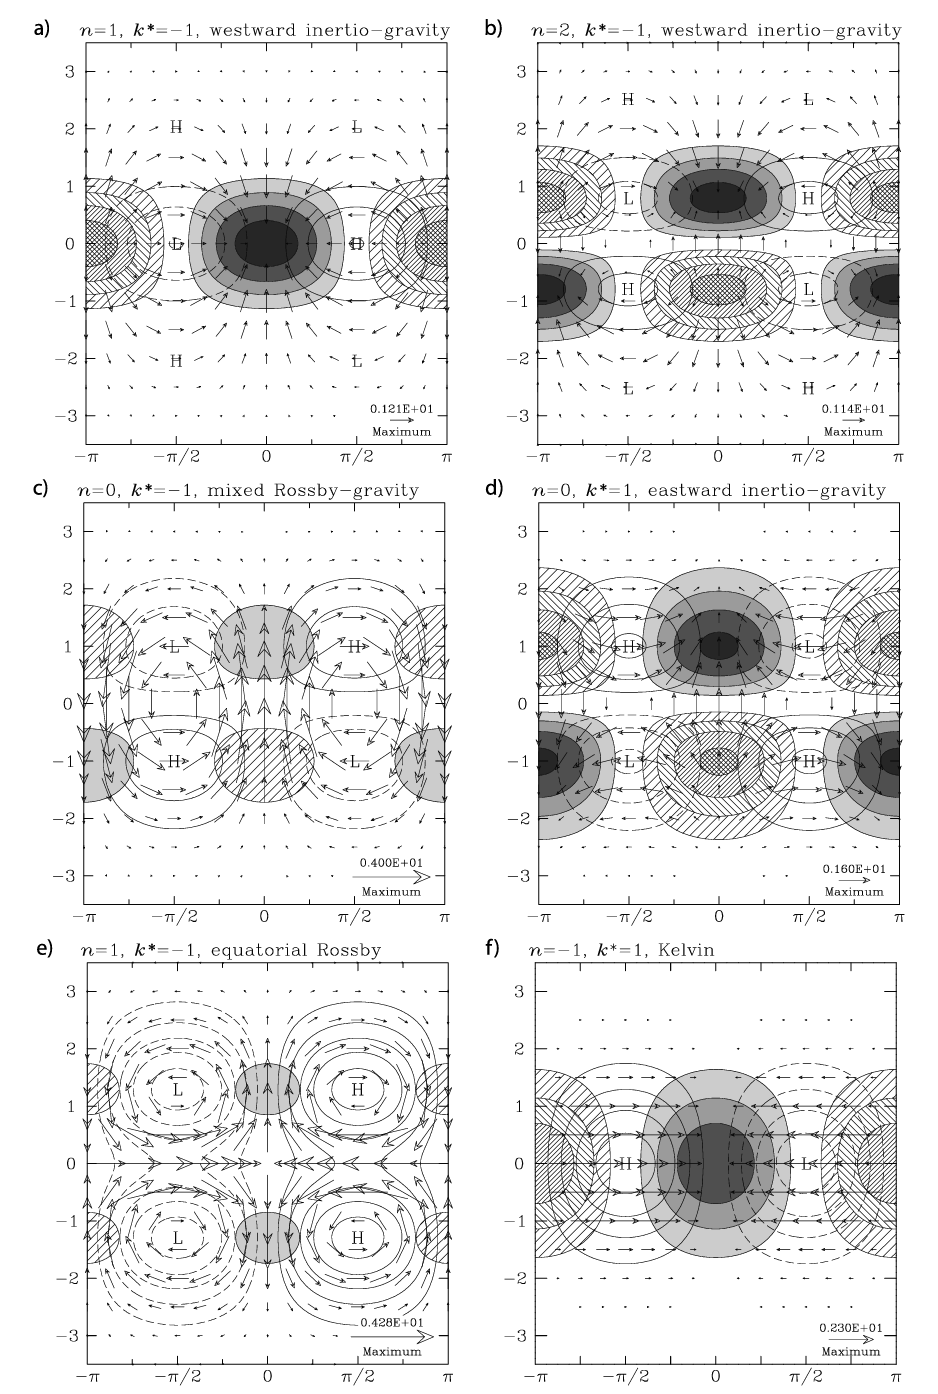
\includegraphics[width=0.9\linewidth]{assets/equatorial_modes.png}
  \caption{典型赤道波模态的水平结构示意图。
    (a,b) 西向惯性重力波（分别对应不同的经向模态指数 $\modenum$）；
    (c) 混合 Rossby-重力波（MRG/Yanai 模态，$\modenum=0$）；
    (d) 东向惯性重力波；
    (e) 赤道 Rossby 波；
    (f) 赤道 Kelvin 波。
    图中箭头表示水平风场矢量分布，阴影与等值线分别代表位势高度（或温度）扰动的幅度与相位结构，
    共同刻画了不同赤道波模态在赤道波导内的典型空间组织形式。
    该图引用自 \citep{kiladisConvectivelyCoupledEquatorial2009}。}
  \label{fig:equatorial_modes}
\end{figure}

对于 $\modenum \geq 1$ 的模态，经向速度振幅取为谐振子本征函数 $\complexamp{v}(y) = \hfunc{\modenum}(y)$，这在图 \ref{fig:equatorial_modes}(a,b,e) 中表现为具有明确节点数的经向结构，且随 $\modenum$ 增大，流场的经向复杂度相应提高。
由式 \eqref{eq:qr_solution} 与 \eqref{eq:qr_def}，并利用梯算子对厄米函数的作用关系 \eqref{eq:ladder_action}，纬向速度与位势高度的经向结构可显式表示为：
\begin{align}
    \complexamp{u}(y) &= -\frac{\ii}{\sqrt{2}}
    \left[
    \frac{\sqrt{\modenum+1}\,\hfunc{\modenum+1}(y)}{\frequency - \wavenum}
    + \frac{\sqrt{\modenum}\,\hfunc{\modenum-1}(y)}{\frequency + \wavenum}
    \right]
    \label{eq:u_meridional} \\
    \complexamp{\gravpotential}(y) &= -\frac{\ii}{\sqrt{2}}
    \left[
    \frac{\sqrt{\modenum+1}\,\hfunc{\modenum+1}(y)}{\frequency - \wavenum}
    - \frac{\sqrt{\modenum}\,\hfunc{\modenum-1}(y)}{\frequency + \wavenum}
    \right]
    \label{eq:phi_meridional}
\end{align}

上述表达式表明，尽管经向速度 $\complexamp{v}$ 仅包含单一的 $\modenum$ 阶厄米函数，纬向速度 $\complexamp{u}$ 与位势高度 $\complexamp{\gravpotential}$ 却由相邻的 $\hfunc{\modenum\pm 1}$ 的线性组合构成。
这种模态耦合直接反映了赤道 $\beta$ 效应下动量方程与连续方程之间的内在联系，也是赤道波区别于中高纬行星波的重要特征。
值得强调的是，对于给定的经向模态指数 $\modenum$，不同类型的赤道波动（如惯性重力波、Rossby 波及混合 Rossby-重力波）虽然具有相同的经向节点数结构，但由于其本征频率 $\frequency$ 不同，式 \eqref{eq:u_meridional}--\eqref{eq:phi_meridional} 中各项的相对权重发生变化，从而导致纬向风场与位势场在定量结构上的显著差异。
这一差异在图 \ref{fig:equatorial_modes} 中表现为不同模态下流线形态与高低压区分布方式的系统变化。

\subsection{色散关系的有量纲形式与观测验证}
\label{subsec:dimensional_form}

为便于与实际大气观测进行定量比较，需要将上述无量纲形式的色散关系恢复为有量纲表达。
无量纲频率与波数与其有量纲对应量之间满足：
\begin{equation}
    \frequency_{\text{dim}} = \frequency\sqrt{\ceq\rossby},
    \qquad
    \wavenum_{\text{dim}} = \wavenum\sqrt{\rossby/\ceq}
    \label{eq:dimensional_conversion}
\end{equation}

其中 $\ceq = \sqrt{\gravityconst\eqdepth}$ 为等效浅水波速，$\rossby$ 表示赤道 $\beta$ 参数。
在该尺度变换下，惯性重力波的有量纲色散关系可写为：
\begin{equation}
    \frequency_{\text{dim}}^2 \approx \wavenum_{\text{dim}}^2\ceq^2 + (2\modenum + 1)\rossby\ceq
\end{equation}

其中第一项对应重力波的传播效应，第二项体现赤道 $\beta$ 效应引入的有效惯性频率，其大小由经向模态指数 $\modenum$ 所控制。
相应地，赤道 Rossby 波在有量纲形式下满足：
\begin{equation}
    \frequency_{\text{dim}} \approx -\frac{\rossby\wavenum_{\text{dim}}}{\wavenum_{\text{dim}}^2 + (2\modenum + 1)\rossby/\ceq}
\end{equation}

该色散关系清楚表明 Rossby 波的低频特性及其始终向西传播的性质。
分母中的第二项反映了赤道波导对经向结构的约束作用，当经向模态阶数增大时波动的相速度显著减小，体现出高阶模态传播效率的系统性降低。

\begin{figure}[htbp]
  \centering
  \fbox{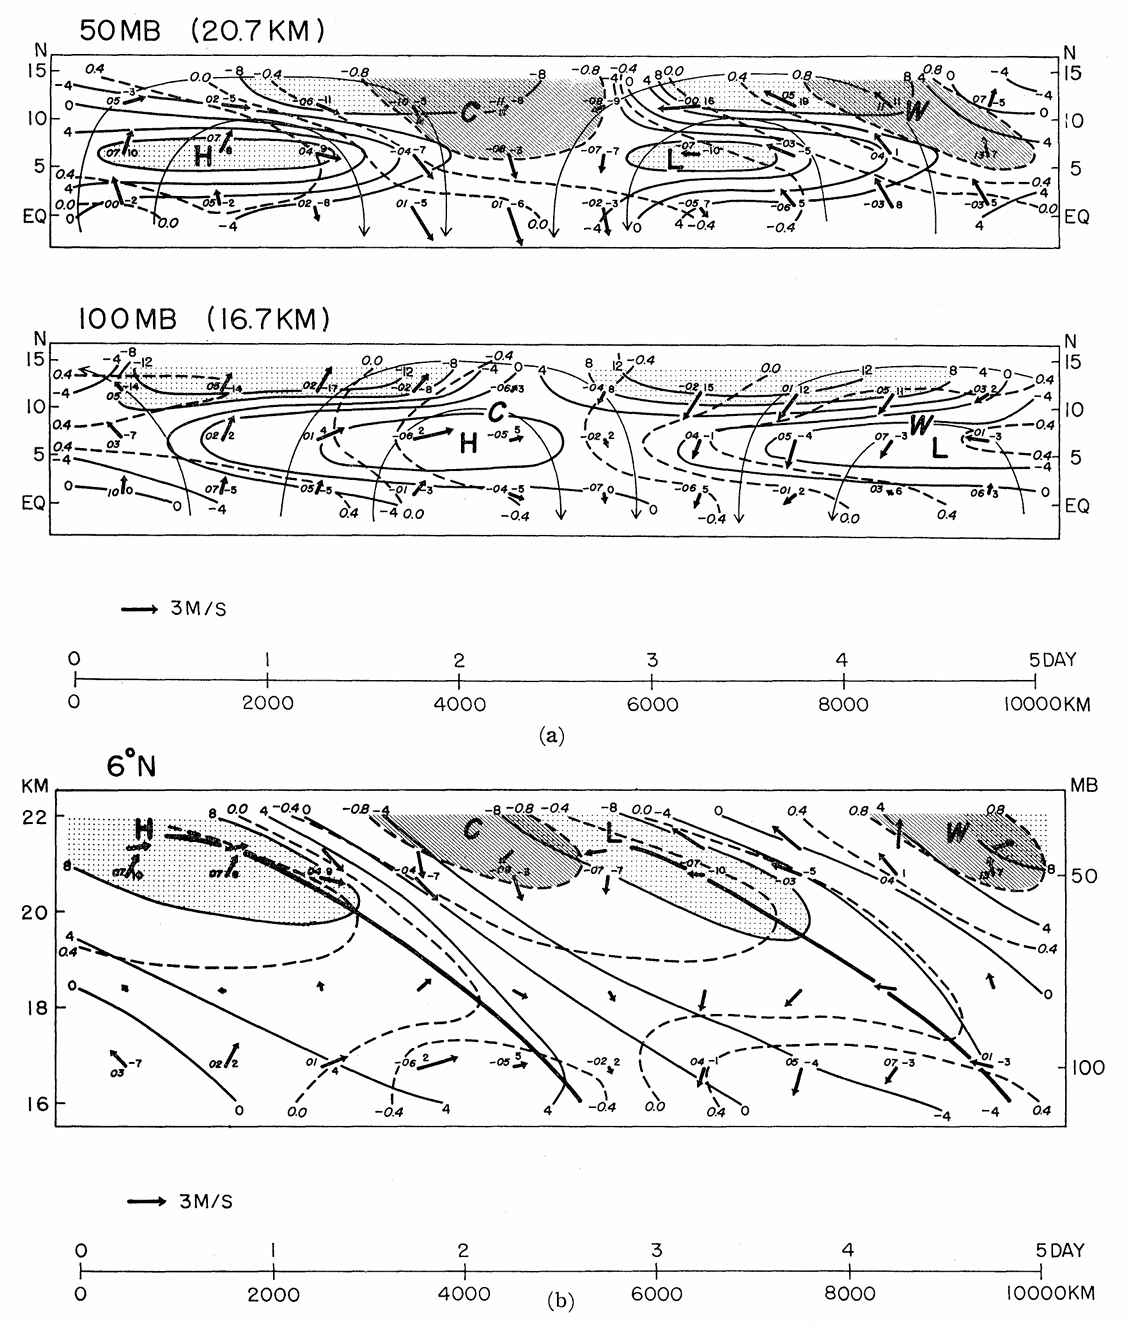
\includegraphics[width=0.9\linewidth]{assets/maruyama_fig15.png}}
  \caption{平流层中混合 Rossby-重力波（MRG/Yanai 模态）的三维结构示意（观测重建）。
  (a) 水平结构显示扰动在赤道附近呈现显著的赤道束缚特征，并以涡旋型风场与位势（或温度）异常相伴随；
  (b) 纬向-高度剖面中相位线随高度向西倾斜，表明波动具有向上传播的垂直结构特征。
  该图引用自 \citep{Maruyama1967}。}
  \label{fig:maruyama_fig15}
\end{figure}

上述有量纲色散关系为理论结果与实际大气观测之间建立了直接的对应桥梁。
平流层观测中识别出的混合 Rossby-重力波，在水平结构、传播方向及垂直相位倾斜特征上，均与干大气赤道波理论的预言保持高度一致。
图 \ref{fig:maruyama_fig15} 所示的观测结果 \citep{Maruyama1967} 清楚展示了该类波动在真实大气中的三维结构特征：其水平风场与位势（或温度）异常在赤道附近呈现出明显的束缚结构，并伴随典型的旋转型环流形态，这与理论中由厄米函数描述的经向模态分布高度一致；同时，垂直剖面中相位随高度系统性倾斜，表明波动具有清晰的向上传播特征，与色散关系所预言的垂直传播性质和传播方向完全相符，为 Matsuno 赤道波理论提供了直接的观测支持。
关于赤道波动观测的更详细综述可参见 \citep{kiladisConvectivelyCoupledEquatorial2009}。

\subsection{对流耦合赤道波与等效深度的修正}
\label{subsec:heating_effect}

前述干大气理论成功解释了平流层中观测到的赤道波动，但无法解释对流层观测到的对流耦合赤道波（convectively coupled equatorial waves, CCEWs）的慢传播特性。
观测表明，CCEWs 的相速度约为干波预测值的 $1/2$ 至 $1/3$，这一显著偏差暗示非绝热加热 $\nonadheat$ 在热带对流层波动中起关键作用 \citep{kiladisConvectivelyCoupledEquatorial2009}。
本小节将湿过程效应纳入第 \ref{sec:framework} 节建立的理论框架，讨论其对波动传播特性的修正。

回顾热力学方程 \eqref{eq:thermo_phi}：
\begin{equation}
    \pde{}{\timevar}\left(\pde{\gravpotential}{z}\right) + \bvfreq^2 w = \nonadheat
    \label{eq:thermo_with_Q}
\end{equation}

当 $\nonadheat = 0$ 时，可消去 $w$ 得到组合方程 \eqref{eq:combined_continuity}，进而定义自伴的垂直算子 $\vertop$。
然而，当 $\nonadheat \neq 0$ 且其垂直结构与本征函数族 $\{\vertfunc_j(z)\}$ 不一致时，第 \ref{subsec:separation} 小节中建立的垂直-水平分离将被破坏，不同垂直模态之间产生耦合，分离变量方法失效。

为恢复代数结构的可处理性，采用 \citep{lindzenWaveCISKTropics1974} 提出的 Wave-CISK 参数化，即式 \eqref{eq:heating_param}：
\begin{equation}
    \nonadheat = -\moistparam\bvfreq^2 w
    \label{eq:wave_cisk_repeat}
\end{equation}

该参数化假设非绝热加热率与垂直上升运动强度成正比，其物理基础是热带大气中低层辐合（$w > 0$）触发深对流从而释放潜热的机制。
将参数化 \eqref{eq:wave_cisk_repeat} 代入热力学方程 \eqref{eq:thermo_with_Q}，可得：
\begin{equation}
    \pde{}{\timevar}\left(\pde{\gravpotential}{z}\right) + (1 - \moistparam)\bvfreq^2 w = 0
\end{equation}

该式形式上与干大气情形 \eqref{eq:thermo_phi} 完全一致，只是 Brunt-Vaisala 频率的平方被替换为了有效静力稳定度：
\begin{equation}
    \bvfreq_{\mathrm{eff}}^2 \equiv (1 - \moistparam)\bvfreq^2
    \label{eq:effective_stability}
\end{equation}

因此，Wave-CISK 参数化等价于将 $\bvfreq^2$ 替换为 $\bvfreq_{\mathrm{eff}}^2 < \bvfreq^2$，即降低大气的有效稳定度。
由于热力学方程恢复了标准形式，第 \ref{sec:framework} 节的全部推导仍然成立，只需将 $\bvfreq$ 替换为 $\bvfreq_{\mathrm{eff}}$。

在此参数化下，修正的垂直算子为：
\begin{equation}
    \vertop_{\mathrm{eff}} \equiv \frac{1}{\density_0(z)}\pde{}{z}\left(\frac{\density_0(z)}{\bvfreq_{\mathrm{eff}}^2(z)}\pde{}{z}\right) = \frac{1}{1 - \moistparam}\vertop
    \label{eq:effective_operator}
\end{equation}

其中最后一个等号假设 $\moistparam$ 不依赖于高度 $z$。
由于 $\vertop_{\mathrm{eff}} = \vertop/(1-\moistparam)$，本征函数 $\vertfunc_j(z)$ 保持不变，但本征值发生改变。
若干大气本征方程为 $\vertop\vertfunc_j = -\vertfunc_j/(\gravityconst\eqdepth_j)$，则修正的本征方程给出有效等效深度：
\begin{equation}
    \eqdepth_{\mathrm{eff}} = (1 - \moistparam)\eqdepth
    \label{eq:effective_equivalent_depth}
\end{equation}

相应地，有效波速为：
\begin{equation}
    \ceq_{\mathrm{eff}} = \sqrt{\gravityconst\eqdepth_{\mathrm{eff}}} = \sqrt{1 - \moistparam}\cdot\ceq
    \label{eq:effective_wave_speed}
\end{equation}

当 $\moistparam = 0.75$ 时，$\ceq_{\mathrm{eff}} = 0.5\ceq$，波速减半。
这与观测到的 CCEWs 相速度约为干波预测一半的结果定性一致 \citep{kiladisConvectivelyCoupledEquatorial2009, lindzenWaveCISKTropics1974}。

\subsection{湿大气中的色散关系}
\label{subsec:modified_dispersion}

固定无量纲化尺度为干大气值 $\Leq_0 = \sqrt{\ceq_0/\rossby}$，$\Teq_0 = 1/\sqrt{\ceq_0\rossby}$，其中 $\ceq_0 = \sqrt{\gravityconst\eqdepth}$。
在此尺度下，有效波速的无量纲值为 $\ndim{\ceq}_{\mathrm{eff}} = \ceq_{\mathrm{eff}}/\ceq_0 = \sqrt{1 - \moistparam}$。
无量纲连续性方程 \eqref{eq:nondim_phi} 变为：
\begin{equation}
    \pde{\gravpotential}{\timevar} + (1 - \moistparam)\left(\pde{u}{x} + \pde{v}{y}\right) = 0
\end{equation}

重复第 \ref{subsec:matsuno_dispersion} 小节的推导，设 $\complexamp{v} = \hfunc{\modenum}(y)$，得到代数方程：
\begin{equation}
    \frac{\modenum + 1}{\frequency - (1 - \moistparam)\wavenum} + \frac{\modenum}{\frequency + (1 - \moistparam)\wavenum} = \frac{\frequency}{1 - \moistparam}
    \label{eq:algebraic_moist}
\end{equation}

定义重新标度的变量：
\begin{equation}
    \ndim{\frequency} \equiv \frac{\frequency}{\sqrt{1 - \moistparam}}, \quad \ndim{\wavenum} \equiv \wavenum\sqrt{1 - \moistparam}
\end{equation}

则式 \eqref{eq:algebraic_moist} 化为标准 Matsuno 形式 $\ndim{\frequency}^3 - (\ndim{\wavenum}^2 + 2\modenum + 1)\ndim{\frequency} - \ndim{\wavenum} = 0$。
因此，色散关系的形式保持不变，只是频率和波数作了缩放。
原始变量中的频率为：
\begin{equation}
    \frequency = \sqrt{1 - \moistparam}\cdot\ndim{\frequency}(\ndim{\wavenum})
    \label{eq:frequency_rescaling}
\end{equation}

这一结果表明，湿耦合使所有赤道波的频率按相同的因子 $\sqrt{1-\moistparam}$ 降低，而不改变色散关系的基本结构。
在物理上，Wave-CISK 参数化通过全局降低大气的有效稳定度，对所有模态产生相同比例的修正。
观测约束表明，CCEWs 的相速度约为干波的 $1/2$，对应 $\sqrt{1-\moistparam} \approx 0.5$，即 $\moistparam \approx 0.75$ \citep{kiladisConvectivelyCoupledEquatorial2009}。
此时耦合参数较大，第 \ref{sec:perturbation} 节将发展微扰方法对这一强耦合情形进行更系统的分析。

\subsection{小结}
\label{subsec:chap3_summary}

本节在第 \ref{sec:framework} 节建立的数学框架下，系统分析了赤道波动的本征模态结构。
在干大气近似下，假设 Brunt-Vaisala 频率为常数，垂直本征方程可显式求解，其解表现为振幅随高度指数增长的振荡结构，垂直波数由式 \eqref{eq:vertical_wavenumber} 确定。
刚性盖边界条件导致等效深度形成离散谱，由式 \eqref{eq:equivalent_depth_quantized} 给出；若采用辐射边界条件允许能量向上传播，则等效深度转而构成连续谱。
固定垂直模态后，水平结构满足 Matsuno 色散关系 \eqref{eq:matsuno_dispersion}，每一组 $(\wavenum, \modenum)$ 对应三类动力学上不同的波动分支，包括两支惯性重力波和一支赤道 Rossby 波。
赤道 Kelvin 波由于其经向速度恒为零而需作为特殊模态单独处理，其特征是严格非频散并仅允许向东传播。
干大气理论成功解释了平流层中观测到的 Kelvin 波、混合 Rossby-重力波及惯性重力波等基本模态。

然而，该理论无法解释对流层中对流耦合赤道波所表现出的慢传播特性。
通过引入 Wave-CISK 参数化 \eqref{eq:wave_cisk_repeat}，湿过程效应可等价地理解为降低大气的有效静力稳定度，从而使有效等效深度减小为 $(1-\moistparam)\eqdepth$，波速相应降低为 $\sqrt{1-\moistparam}\cdot\ceq$。
色散关系的形式保持不变，但所有模态的频率按统一因子缩放。
这一结果定性地解释了 CCEWs 的慢传播现象，表明观测到的对流耦合波动可以理解为干波本征模态在热力加热作用下的连续变形，而非全新的动力学模态。
第 \ref{sec:perturbation} 节将在此基础上发展系统的微扰方法，进一步分析加热对波动性质的修正。
